\chapter{Réalisations techniques}
Comme énoncé dans la première partie de ce mémoire, nus allons concentrer notre travail sur la sécurisation des 
développements applicatifs jusqu'à leur déploiement. Nous aborderons donc des sujets tels que la création de deux 
procédures de sécurité, l'outillage des équipes ainsi que la réalisation de diverses évaluations de sécurité.

\section{Une première approche du DevSecOps}
Rapidement évoqué dans l'état de l'art, l'équipe de \ac{SSI} a entamée ,dès le quatrième semestre de 2018, un premier 
travail d'intégration de sécurité informatique dans les développements au travers de la mise en place d'un processus 
\emph{Security By Design}.

Ce processus, centré en son cœur sur l'accompagnement de \emph{Security Champions}\footnote{Un 
\emph{Security Champion} est un ambassadeur de la \ac{SSI} dans les équipes projets.}, vise à faciliter le questionnement
et  les réflexions sur les sujets de \ac{SSI} dans les équipes projets. Représentés par des responsables produit, des 
développeurs ou opérationnels, ils favorisent les échanges entre les équipes projets et l'équipe de \ac{SSI} en servant 
de réels points de liaisons pour ces dernières.

Grâce au travail des \emph{Security Champions}, le nombre de demande d'audit technique et de conseils d'architecture
a progressivement augmenté tout au long de l'année 2019. L'équipe s'est donc retrouvé à réaliser plusieurs audits par 
mois sur l'année 2019 là où elle n'en réalisait qu'un tous les deux mois en moyenne en 2018. J'ai par ailleurs eu le 
plaisir de m'occuper d'une majorité de ces qualifications sécurité.

C'est d'ailleurs sur cette même période qu'un projet de personnalisations des règles du \ac{SAST} (SonarQube) exploité 
par JCDecaux a été lancé. Ces personnalisations, réalisées en deux temps, visaient à créer plusieurs profils d'analyse 
pour chaque langage de programmation utilisé dans l'entreprise, tout en réduisant le bruit généré par des règles 
remontant trop de faux positif.

Grace à ces actions, portés tant auprès du Groupe qu'auprès de ses filiales, l'équipe de \ac{SSI} s'est rapproché un peu
plus de son objectif de sécurisation des applications développées en interne. Cette approche proactive et non plus 
réactive de sécurisation a notamment permis de réduire considérablement le nombre d'applications rejetées à la suite d'une 
qualifications sécurité pré-déploiement en production.

Nous passions donc d'une méthodologie agile \emph{DevOps} à une méthodologie \emph{DevSecOps}.

\newpage

\section{Les audits : quel processus pour quel résultat}
Depuis 2019, nous (l'équipe de \ac{SSI}) avons observé une nette augmentation du nombre de qualifications sécurité réalisées
aux profits des projets de développement. Cette augmentation, bien que bénéfique à l'objet de l'équipe, a eu pour effet 
de mettre en évidence divers problèmes ans l'organisation et la réalisation de ces audits.
\newline Il nous arrivait encore à cette période de devoir interrompre la publication de certaines applications n'étant 
pas qualifiées, faute de procédures explicites et partagées à toutes les équipes de JCDecaux. Nous avons donc commencé à 
travailler sur la question avec l'aide de quelques équipes de la \ac{DSI} France.

La première réalisation dans cette quête de structure à été la définition claire et précise des points de contrôle et 
des vulnérabilités recherchées sur les applications. Ces points de contrôle sont fortement inspirés par l'OWASP Top ten
\autocite{owasp_top10_2017} et sont formulés dans un tableur servant à faire leur suivi durant l'audit. Chacun est 
ensuite associé à plusieurs états (testé ou non, risque et application de correctifs) ainsi qu'un commentaire le cas 
échéant.

À cette liste de points de contrôle est ensuite adossé une revue du projet sur SonarQube (note \ac{SAST}) et de la 
classification des entrées remontées par l'outil. Cette étape nous permets de prendre la mesure de la qualité du code de 
l'application auditée, mais aussi du niveau d'attention apporté par l'équipe de développement à son application.
\newline Nous avons en effet constaté que les projets ayant le plus de vulnérabilité et erreur de code remonté par 
SonarQube était géré par des équipes ayant peu d'intérêt dans le contrôle qualité de leur code.
\newline Ce même type de revue est réalisé le niveau de vulnérabilité des conteneurs pour les applications concernées, 
mais nous reviendrons sur ce sujet plus tard.

Nous avons par la suite commencé à travailler sur la définition des livrables et des points abordés durant la réunion de
restitution. Il est important de noté que ces livrables se limitaient jusque-là à une simple liste de vulnérabilités
ordonnées en fonction de leur criticité et sans démonstration ou explication du chemin d'attaque.
\newline  La mise en place d'une restitution appropriée et argumentée de l'audit à permis de déceler quelques 
méconnaissance dans plusieurs équipes (notamment vis-à-vis du framework IAM du groupe) et sert souvent de point de départ 
à l'accompagnement des équipes entament leur migration vers le DevSecOps.

Voilà donc comment fonctionnait le processus d'audit applicatif entre 2019 et 2020. 
\newline Cependant, ce processus étant tacite et non-formalisé (la culture de l'orale étant encore très fort chez 
JCDecaux), plusieurs départs et changements de postes l'ont mis à mal.

C'est pourquoi nous avons entrepris de formuler ce processus dans un langage commun (ici le \ac{BPMN}) afin de le partager
aux équipes impliquées dans celui-ci. Nous en avons profité pour intégrer quelques prérequis facilitant l'organisation 
de l'audit technique et la création de garde-fous.

\newpage

Le processus d'audit est donc représenté sous la forme de deux diagrammes : le premier décrivant le fonctionnement 
générale de l'audit et des différents échanges entre l'équipe de développement et l'équipe de \ac{SSI}; le second 
décrivant les actions techniques réalisées durant l'audit.

\begin{figure}[h]
    \centering
    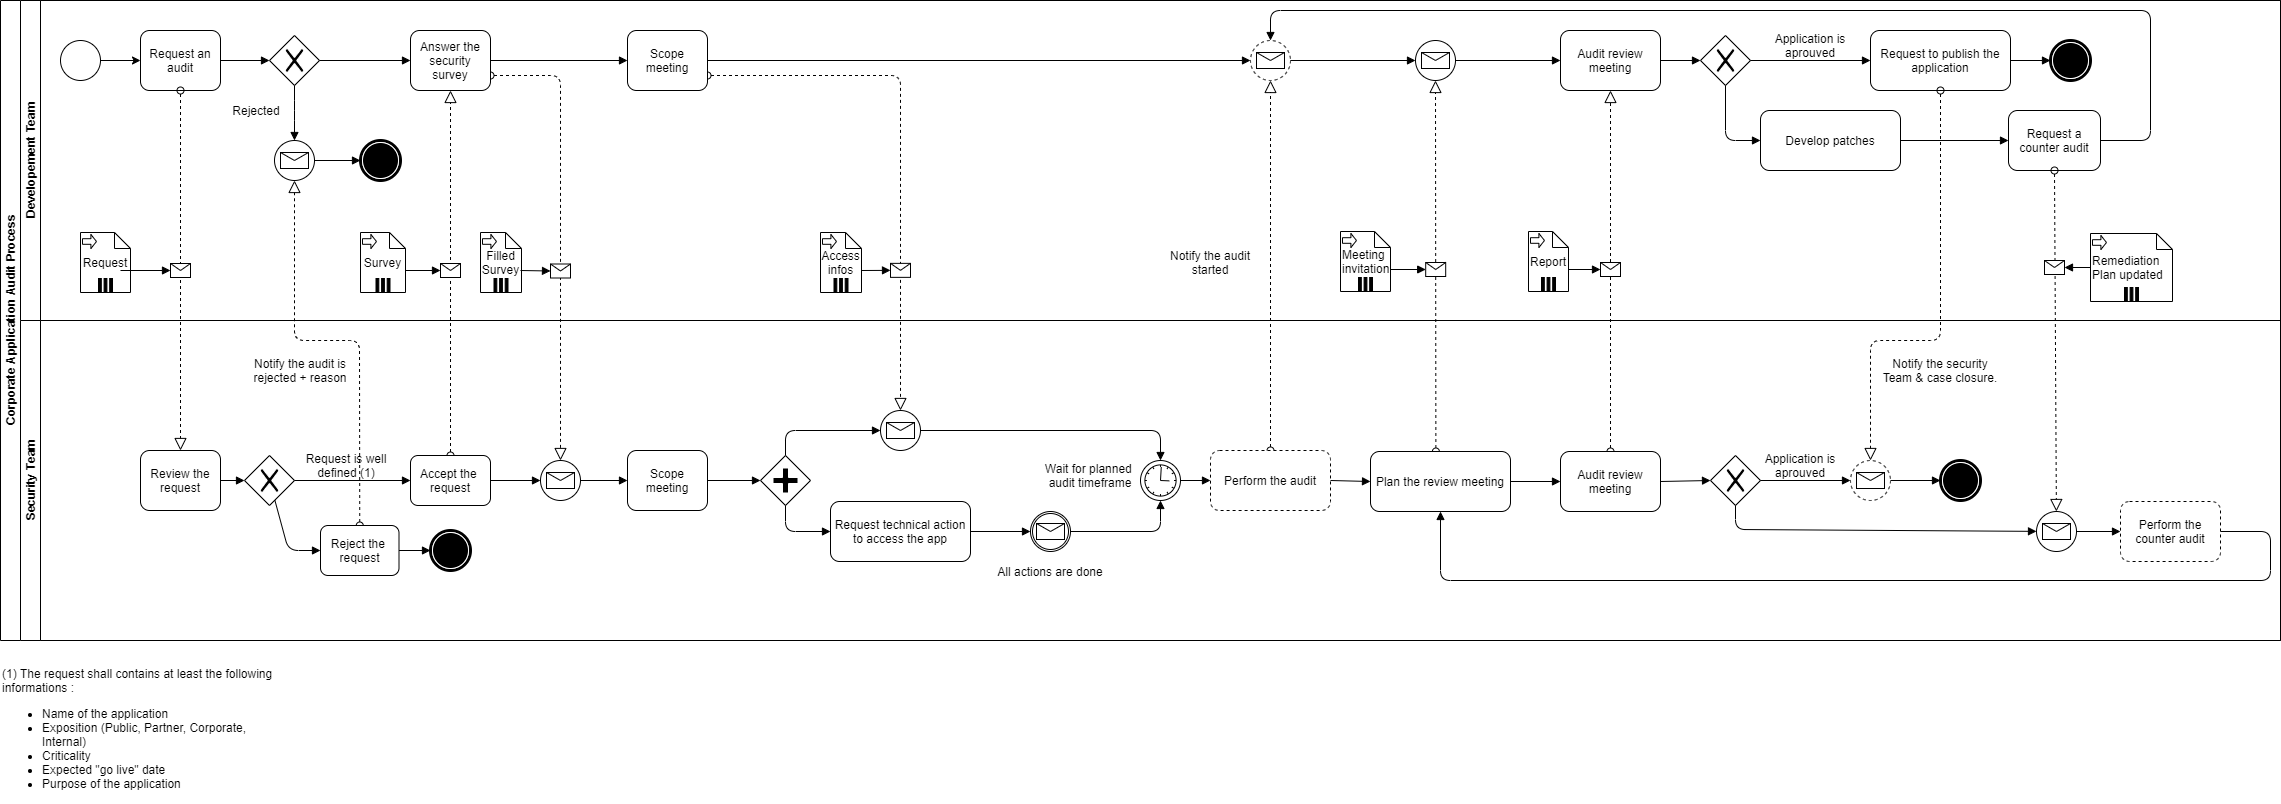
\includegraphics[width=\linewidth]{resources/img/process_audit.png}
    \caption{Processus de l'audit de sécurité d'une application}
\end{figure}

\begin{figure}[h]
    \centering
    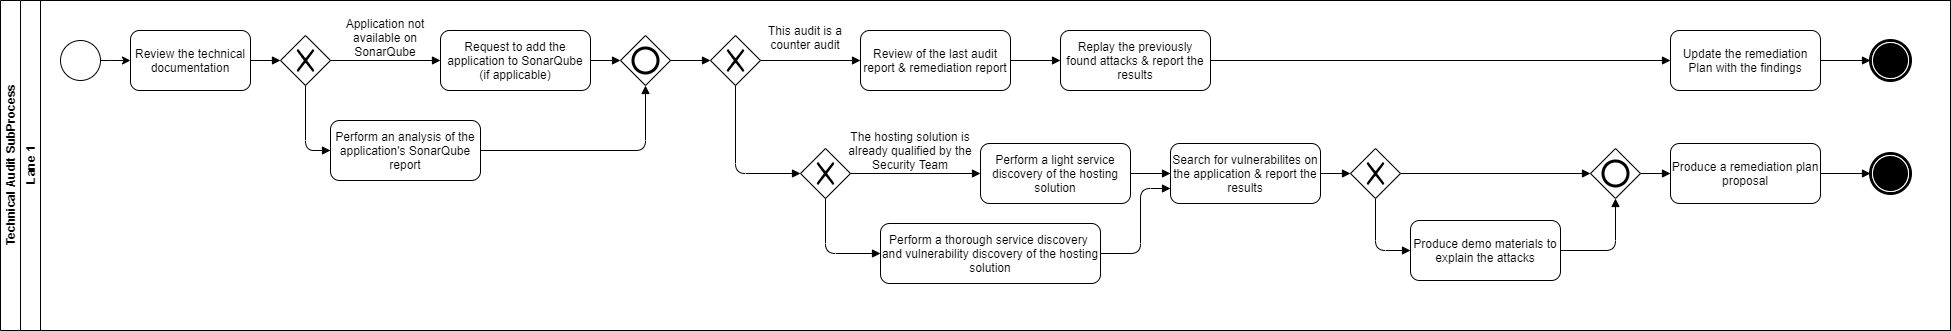
\includegraphics[width=\linewidth]{resources/img/technical_audit_subprocess.png}
    \caption{Processus fils de l'audit de sécurité d'une application : actions techniques}
\end{figure}
\begin{center}
    \colorbox{gray!15}{Ces deux diagrammes étant relativement complexes, vous les retrouverez en annexes}
\end{center}

Nous trouvons donc dans ce processus nouvellement formalisé l'ensemble des éléments précédemment évoqués avec l'ajout 
de quelques nouveautés nous permettant de mieux préparer l'audit. C'est ainsi qu'est intégré un questionnaire visant à
fournir à l'équipe de \ac{SSI} des informations supplémentaires sur la nature de l'application devant être audité ainsi 
que les éventuelles contraintes temporelles.

Ce processus étant en place dans sa version définitive depuis Avril 2021, nous observons une amélioration progression des 
conditions d'organisation des audits techniques, notamment sur les éléments de contexte relatif aux applications devant 
être audités.
Il s'agissait en effet d'un certain point de friction de septembre 2020 suite au départ d'une de nos collaboratrices.

\newpage

\section{Inventaire et gestion de la sécurité des conteneurs}
Si la sécurité des applications est un sujet ayant fait l'office d'une certaine attention depuis ces trois dernières années
au sein du Groupe JCDecaux, la sécurité des conteneurs n'a pas eu cette chance faute de temps.
\newline Pour rappel, cette question n'a été abordée que brièvement lors des audits applicatifs jusqu'à la demande de 
mise en production de la plateforme \ac{K8S} et son audit par XMCO.

Le premier aspect de sécurité des conteneurs à adresser porte sur la création et le maintient d'un inventaire exhaustif
des \emph{Pods} en exécution sur les clusters et de leur état de vulnérabilité. S'il nous était possible d'extraire à la
main cet inventaire depuis un cluster \ac{K8S}, leur multiplication à la suite au cloisonnement de 
l'infrastructure a rendu la chose bien plus compliquée. Il nous faut donc nous équiper en conséquence.

\subsection{Recherche d'outils}
Nous avons commencé à recherche des outils capables de nous fournir les informations nécessaires au suivi opérationnel 
des vulnérabilités des \emph{Pods} en fonctionnement. 

Cette recherche avait pour contraintes les éléments suivants :
\begin{itemize}
    \item Fonctionnement multicluster
    \item WebApplication pour la remontée des informations
    \item Mise à jour de l'inventaire automatique et journalière
    \item Export de rapport managérial
\end{itemize}

Quatre solutions correspondaient donc à notre besoin :
\begin{itemize}
    \item Le projet klustair (www.klustair.com)
    \item Le service de sécurité Kubernetes d'Aqua (www.aquasec.com)
    \item Le service de sécurité Kubernetes d'Alcide (www.alcide.io)
    \item Le service de scanner de vulnérabilité de Snyk (www.snyk.io)
\end{itemize}

Après une rapide analyse de ces solutions (voir tableau \ref{tab:sectoolscompkub}), nous constatons que si la solution 
\emph{Klustair} semblait correspondre au besoin, des fonctionnalités importantes sont manquantes. Notre choix devra donc
s'orienter vers les solutions commerciales.

Cependant, compte tenu de la crise de la COVID-19 et du verrouillage des budgets nous ne pouvons plus lancer de projet à 
plus de 5 000€ dans l'accord du \ac{DAF}. Or, dans le cas des trois solutions restantes, la facture s'élèverait à minima
à \linebreak 25 000€ annuel.

Nous nous trouvons donc avec un dilemme : soit intégrer une solution peu sécurisée et remplissant une portion de nos 
besoin, soit entamer une négociation avec la direction afin de débloquer des budgets et plus que probablement se voir 
refuser la proposition.

\newpage 

\begin{table}[h]
    \begin{center}
            \begin{tabular}{p{5cm}|llll}
                                                                & \textbf{Klustair} & \textbf{Aqua}              & \textbf{Alcide} & \textbf{Snyk}              \\
                \toprule
                \textbf{Coût license}                            & OpenSource        & \textgreater 2 000€ / mois & Inconnu         & \textgreater 3 000€ / mois \\
                \hline
                \textbf{Fonctionnement}                          & Auto-hébergé      & SaaS                       & SaaS            & SaaS                       \\
                \hline
                \textbf{Authentification}                        & Non               & Oui                        & Oui             & Oui                        \\
                \hline
                \textbf{Intégration registre Cloud}              & Oui               & Oui                        & Oui             & Oui                        \\
                \hline
                \textbf{Inventaire de Pods en fonctionnement}    & Oui               & Oui                        & Oui             & Oui                        \\
                \hline
                \textbf{Scanner de vulnérabilité}                & Oui               & Oui                        & Oui             & Oui                        \\
                \hline
                \textbf{Scanner de configuration / secrets}      & Possible          & Oui                        & Oui             & Oui                        \\
                \hline
                \textbf{Analyse de l'environnement d'execution}  & Non               & Oui                        & Oui             & Oui                        \\
                \hline
                \textbf{Export de rapport}                       & Non               & Non                        & Oui             & Oui                        \\
                \hline
                \textbf{Fréquence de mise à jour}                & Journalière       & Par heure                  & Par heure       & Par heure                 
            \end{tabular}
            \caption{Comparaison des produits de sécurité pour Kubernetes}
            \label{tab:sectoolscompkub}
    \end{center}
\end{table}

La solution à ce problème arrive cependant lorsqu'en Avril 2021 notre fournisseur de scanner de vulnérabilité 
d'infrastructure annonce l'intégration de fonctionnalités dédier à Kubernetes dans InsightVM, la solution déjà utilisée 
par l'équipe \ac{SSI}.

\subsection{Gestion de la sécurité des clusters avec InsightVM}
Après une rapide évaluation de faisabilité et expérimentation des fonctionnalités nouvellement intégrées, nous prenons 
contact avec l'éditeur pour obtenir quelques informations supplémentaires sur les recommandations d'implémentations et 
la tarification des fonctionnalités. Aspect intéressant dans notre situation : seul le nombre d'agent de collecte déployé
est comptabilisé dans le nombre d'IP associé à la licence, le reste des fonctionnalités étant intégrées à celle souscrite
par JCDecaux.
\linebreak Cet entretien permet de confirmer le mode de fonctionnement l'agents de collecte, ainsi que des actions qu'il 
effectue sur le cluster. Le fonctionnement  de l'agent et son intégration sur nos clusters est par ailleurs décrit dans 
un diagramme ci-après (voir diagramme \ref{figure:k8sscannerarchi}).

Suite à cet entretien, nous effectuons quelques ajustements sur la configuration de l'agent et le déployons
sur l'ensemble des clusters \ac{npr}. Ce déploiement sur six clusters distincts vis à évaluer l'exploitabilité de la 
plateforme Cloud Security\footnote{Plateforme SaaS de Rapid7 InsighVM dans laquelle est remonté l'ensemble des 
informations relatives aux registres de conteneur et clusters Kuberntes.} et des informations collectées. 

Lorsque nous analysons les données remontées sur la plateforme, nous constatons quelques erreurs et bugs dans le 
fonctionnement de la plateforme. Nous remontons donc ces points au support de l'éditeur et profitons de l'occasion
pour demander l'ajout de plusieurs évolutions pour la plateforme.
\newline Ces évolutions sont maintenant intégrées dans la feuille de route de l'éditeur. Elles devraient être intégrées 
dans la plateforme Cloud Security d'ici au troisième trimestre de 2021.

\begin{figure}[h]
    \centering
    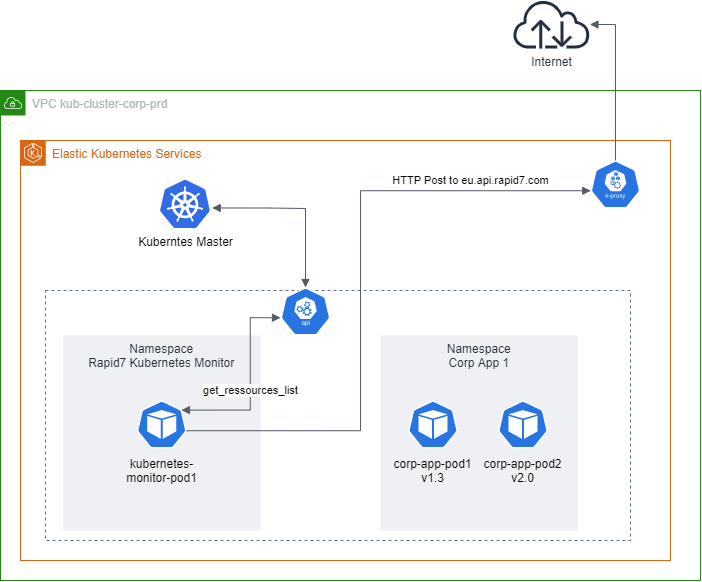
\includegraphics[width=\linewidth]{resources/img/k8s_scanner_archi.png}
    \caption{Schéma de déploiement de kubernetes-monitor sur un cluster Kubernetes}
    \label{figure:k8sscannerarchi}
\end{figure}

\subsection{Première revue de vulnérabilité des conteneurs}

Grâce l'intégration de l'inventaire des clusters Kubernetes sur notre plateforme de gestion opérationnel des vulnérabilités,
nous avons pu réaliser une première revue des images de conteneurs en fonctionnement sur les clusters de \ac{npr}.

Le premier constat que nous pouvons faire est plutôt positif : sur les 183 pod en cours d'exécution sur les clusters 
\ac{K8S}, seul 16 d'entre eux sont issues du registre DockerHub et n'ont donc pas été scanné par Rapid7.
\newline Ces \emph{pods} sont tous localisés dans l'espace de nom \emph{kube-system} et ne peuvent être intégrés sur notre
registre miroirs \ac{AWS} \ac{ECR}.

Cependant, on constate un nombre relativement haut de vulnérabilité (60 en moyenne) pour des conteneurs dont seul les 
paquets sont analysés. De plus, une majorité de ces conteneurs sont basés sur un système d'exploitation Centos 7,
système d'exploitation dont la date de fin de support est incertaine avec le choix de RedHat de migrer vers Centos Stream.

\section{Sécurisation des images}
Nous savons donc, grâce à la première revue de sécurité, qu'une majorité des images de conteneur sont vulnérables et 
nécessitent un travail de remédiation.

Cependant, il nous faut créer une base de prérequis de sécurité commune avec les équipes de développement et 
opérationnel si nous voulons pérenniser les remédiations faites. 
\newline En effet, les procéssus en place pour la production des images (\ie build, qualification, enregistrement sur le
registre, \dots) ne favorise pas la maintenance préventive des images de conteneur. C'est en soit une régression 
vis-à-vis des infrastructures virtualisées.

Il nous faut donc définir des prérequis de sécurité pour les conteneurs et leurs images, ainsi que d'adapter les processus
à ces derniers.

\subsection{Durcissement des images et déploiements}
Cette première phase de sécurisation des images vise à réduire les risques directement portés par l'image du conteneur.

Nous avons donc décrit dans une politique de sécurité dédiée aux conteneurs et à \ac{K8S} un ensemble de prérequis et de 
contraintes. Nous nous sommes pour cela basé sur les recommandations du livre \citetitle{kub_sercuity_rice_2018}
(\citeauthor{kub_sercuity_rice_2018})\autocite{kub_sercuity_rice_2018} et du retour d'expérience de notre équipe 
d'architecture.

\textbf{Prérequis des conteneurs:}
\begin{itemize}
    \item Les images doivent être compilées à partir d'images dites \emph{de base} issues des registres privés de JCDecaux.
    \item Toutes les images doivent être obligatoirement publiée sur les registres privés de JCDecaux, seules sources 
    autorisées sur les clusters \ac{K8S}.
    \item Toutes les versions d'image doivent être désignées par un tag immuable.
    \item Toutes les images doivent faire l'object d'un scan de vulnérabilité à minima toutes les deux semaines.
    \item Une revue des vulnérabilités doit être organisé entre l'équipe de sécurité et les développeurs tous les trois mois.
    L'application des patchs de sécurité est à la charge des équipes de développements.
    \item Aucun conteneur ne doit contenir de secret, mot de passe, token out tuple d'authentification. Ces éléments doivent
    entre obtenu par le biais de la plateforme de centralisation des configurations.
\end{itemize}

\newpage

\textbf{Prérequis de déploiement}
\begin{itemize}
    \item Aucun \emph{pod} ne doit fonctionner avec l'utilisateur \emph{Root}. L'utilisation de \emph{Security Context} 
    permet d'accéder aux fonctionnalités autrement inaccessibles.
    \item Aucun \emph{pod} ne doit monter de ressources propres au nœud de cluster l'hébergeant (\ie 
    \emph{/var/run/docker.socket}, \emph{hostpath}, \dots)
    \item Toute ressource accédée par un \emph{pod} doit être présente dans le même espace de nom ou être explicitement 
    listée dans une \ac{ACL}.
    \item Toute configuration, pour l'espace de nom, d'un pod ou application, doit être distribuée par la plateforme de 
    centralisation des configurations.
    \item Tout script de déploiement doit être hébergé sur les registres internes de JCDecaux(\ie Gitlab, Harbor, \dots).
\end{itemize}

Il sera prochainement intégré à cette politique des restrictions sur le nombre et la nature de vulnérabilité présente 
sur une image devant être déployé. Nous reviendrons sur ce point dans la section \ref{section:revue-vul-img}.
\subsection{Application de la politique}
L'ensemble des prérequis étant maintenant définies dans la politique de sécurité Kubernetes, il nous faut la faire 
appliquer et respecter par les différentes équipes du Groupe.
\newline Pour cela, deux options se présentent à nous : l'application par l'automatisation et l'application par les
processus.

Nous souhaitons réduire au maximum l'impacte de l'intégration de la \ac{SSI} sur l'efficacité des développements, c'est 
pourquoi nous avons fait le choix d'automatiser au maximum les vérifications et validations de conformité.
\newline Cette automatisation est rendue possible grâce à l'utilisation du logiciel \emph{Open Policy Agent Gatekeeper}
sur les clusters.

Cet outil, intégré au contrôleur d'admission \ac{K8S}, permets de définir de façon programmable des contraintes sur les
configurations de déploiements. Ainsi, tout déploiement non conforme à la politique de sécurité se verra automatiquement 
interrompu par l'\emph{OPA Gatekeeper}; la personne à l'origine du déploiement étant immédiatement notifié des 
contraintes non respectées à la suite du blocage.

Nous avons donc fait intégrer l'ensemble des éléments de la politique de sécurité \ac{K8S} dans la base de contrainte d'
\emph{OPA Gatekeeper}. Ces contraintes sont maintenant appliquées sur l'ensemble des clusters du Groupe JCDecaux.

\newpage

\section{Revue des vulnérabilités des images} \label{section:revue-vul-img}
Si nous disposons maintenant d'un inventaire ces conteneurs ainsi que des vulnérabilités les impactant, une gestion 
proactive de la remédiation et plus particulièrement de la gestion des patchs est préférable. C'est d'ailleurs pour cela 
nous l'avons intégrée à la politique de sécurité.

Il nous faut donc mettre en œuvre cette revue de vulnérabilité au sein des équipes impliquées.

\subsection{Ajustement du processus de développement}

Le processus  actuellement en place au sein des équipes de développement du groupe n'impose actuellement pas de contrôle
des vulnérabilités des conteneurs durant la phase de développement. Cela implique donc que cette revue ne se fait qu'à 
l'occasion d'un audit applicatif et que l'application des correctifs n'est faite qu'à la suite de cet audit. 
\newline Il est donc nécessaire d'introduire cette revue de vulnérabilité durant la phase de développement afin de gagner
en efficacité et réduire le niveau de vulnérabilité global des images.

Nous avons donc proposé le processus de développement suivant aux équipes.
\begin{figure}[h]
    \centering
    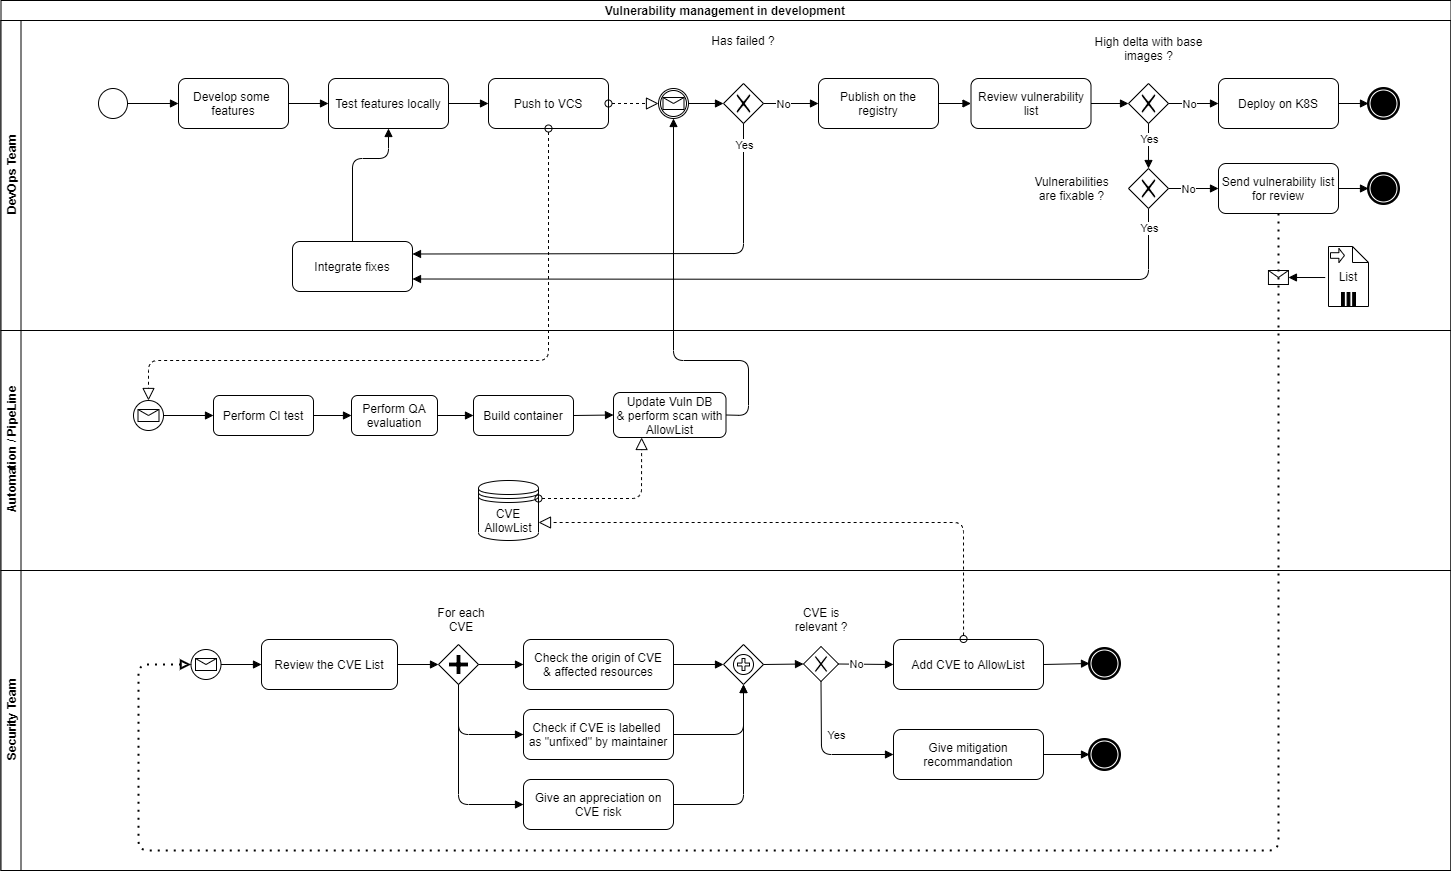
\includegraphics[width=\linewidth]{resources/img/container_image_vuln_mgnt_dev.png}
    \caption{Gestion des vulnérabilités d'image durant le développement}
\end{figure}

Ce nouveau processus intègre donc le scan des images de conteneur par les développeurs, mais aussi de nouveaux éléments tels
que la classification des vulnérabilités et la mise à disposition d'une liste de vulnérabilité donc le risque est accepté
par l'équipe de \ac{SSI}.
\newline L'objectif de ces deux nouvelles actions étant de réduire le bruit généré par le scanner de vulnérabilité durant
le développement, tout en assurant un suivi et contrôle de l'équipe \ac{SSI} sur les vulnérabilités des conteneurs.

\newpage

\subsection{Unification des scanners}
Jusqu'à récemment encore, il existait un certaine disparité entre les scanners de vulnérabilités déployés sur les 
différents pipelines DevOps et ceux utilisés par les registres internes de conteneur. Ainsi, nous nous retrouvions avec 
différentes configurations du scanner \emph{Trivy} sur les pipelines et différentes configurations de \emph{Clair} sur les
registres \emph{\ac{ECR}} et \emph{Harbor}. 
\newline Il devenait donc nécessaire d'unifier outils et configuration pour réaliser au mieux les revues de vulnérabilité.

Après une comparaison de l'efficacité de chaque scanner, nous avons fait le choix de migrer les différents scanners en 
notre possession (hors \ac{ECR} donc) sur une configuration unique de Trivy. Si ce choix peut sembler discutable au vu 
de la sensibilité de l'outil, il l'est beaucoup moins lorsque l'on prend en compte le fait que nous allons déployer une
AllowList pour les vulnérabilités faisant office d'une acceptation de risques.

\subsection{Attribution des vulnérabilités}
Une problématique jusque-là volontairement mise de côté se présente maintenant à nous : à quelle image appartient quelle 
vulnérabilité ?

En effet, nous demandons aux développeurs d'exploiter des images dites \emph{de bases} afin de concevoir leur 
images \emph{applicatives}. Or, ces images \emph{de bases} peuvent porter faire hériter leurs vulnérabilités aux images 
\emph{applicatives} les exploitants.
\newline Il devient donc nécessaire de pouvoir lister de manière dissociée les vulnérabilités propres à chaque image : 
\emph{de bases} ou \emph{applicatives}

Ce problème ne pouvant être réglé avec les outils déjà en place, il nous faut donc en développer un adapté à ce nouveau 
besoin.

\subsection{Développement d'un démonstrateur de classification de vulnérabilité}
Comme évoqué ci-dessus, nous avons donc besoin de concevoir un outil permettant de présenter de manière dissocié les
vulnérabilités d'une image \emph{applicative} des vulnérabilités héritées de son image \emph{de base}.
Nous profitons de ce développement pour intégrer à cet outil la gestion et la génération des AllowList exploités dans les
différents projets.

Par contrainte de temps et de disponibilité de l'équipe de développement infrastructure, j'ai donc entrepris la réalisation 
d'un démonstrateur remplissant l'ensemble de ces besoins. Ce démonstrateur ne présentant aucune mesure de sécurité ni de
gestion suffisante des erreurs, il ne servira qu'à la vérification du principe de fonctionnement et validation du 
processus de classification des vulnérabilités d'image.
\newline L'outil fera l'office d'un "réel" développement courant le quatrième semestre de 2021; il intégrera plus de 
fonctionnalités afin de pouvoir être aussi exploité par les équipes de développement tel que la génération d'une 
AllowList spécifique à une image applicative (intégrant l'ensemble des vulnérabilités de l'image \emph{de base} utilisé 
à l'AllowList). 

\newpage

Ce démonstrateur est encore en développement, la gestion des images applicative étant encore à intégrer, mais les 
premiers retours de l'équipe de \ac{SSI} se veulent encourageants.
\newline Il devrait être terminé et proposer pour qualification vers la mi-juillet.

\vspace{1cm}

\begin{figure}[h]
    \centering
    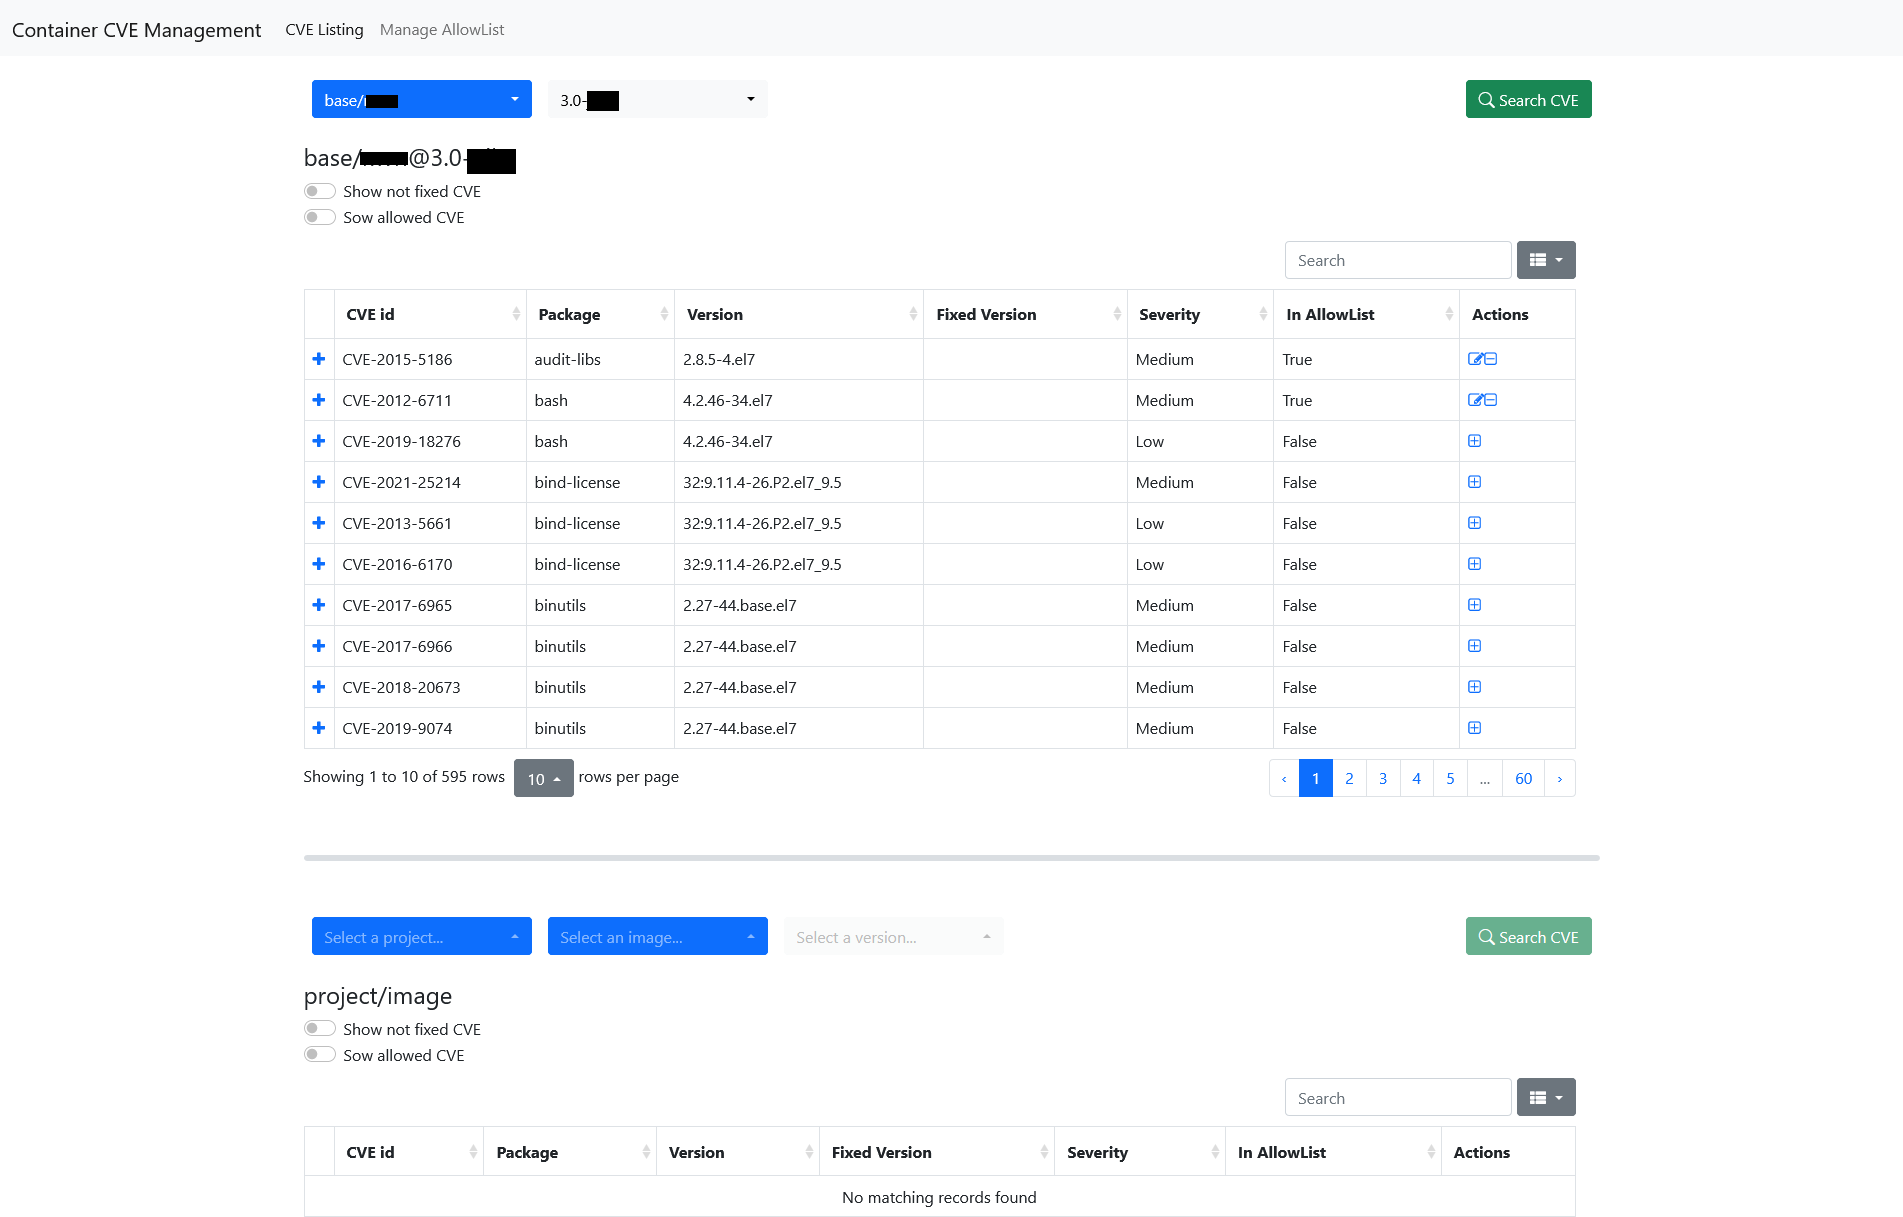
\includegraphics[width=0.9\linewidth]{resources/img/cont_mgnt_listing.png}
    \caption{Liste des vulnérabilités des images en fonction de leur version}
\end{figure}

\begin{figure}[h]
    \centering
    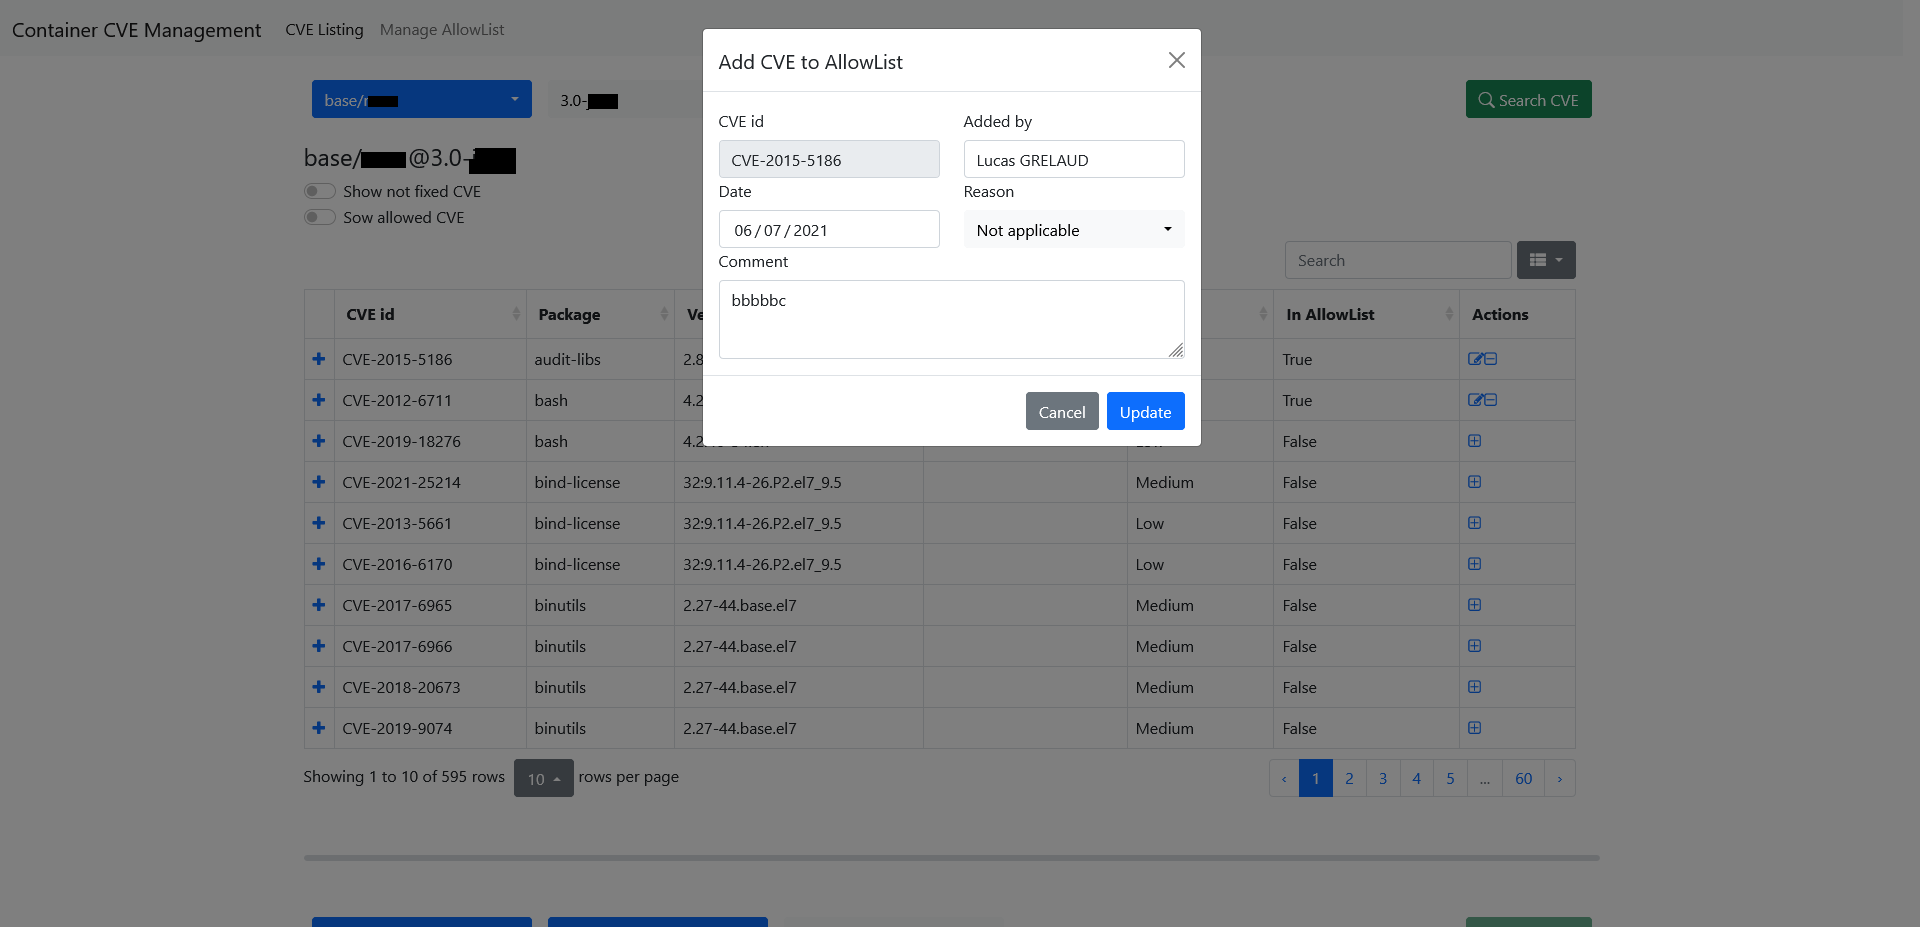
\includegraphics[width=0.9\linewidth]{resources/img/cont_mgnt_add_cve.png}
    \caption{Ajout d'une vulnérabilité à l'AllowList}
\end{figure}
